\chapter{Komponenten und Software-Entwicklung}\label{Komponente}

In diesem Kapitel werden die Hardware-komponente, die in dieser auftretten in Einzelheit dargestellt. Noch dazu wird die Funktionsweise und die Ansteuerung dieser Komponenten erk"art.

\section{STM32L4 Discovery kit}\label{LoRa}

Das STM32L4 Discovery kit ist ein IoT Knoten, womit ein Benutzer Anwendungen mit  direkter Verbindung zu einem oder mehreren Cloud-Server  entwickeln kann. 
Dieses Discovery Kit erm\"oglicht eine Vielzahl von Anwendungen, indem es eine Multikink-Kommunikation (Bleautooth Low energie) mit geringerem Stromverbrauch nutz, Multiway-Erkennung (Erkennung, Umweltbewusstsein) und die kernbasierten   Funktionen der STM32L4-Serie von Arm Cortex\textregistered-M4 (Siehe Abbildung \ref{Node}).

Das STM32L4 hat einen eingebetteten ST-LINK Debugger/Programmieren, Eingebettete Sensoren und viele andere Eingenschaften, die in dem Datenblatt \cite{B-L475E-IOT01A} zu finden sind. Genau wegen der vielfalt an Eingenschaften wurde dieses Board ausgew"ahlt. Man braucht keine Breadbord im Vergleich zu dem Arduino oder dem Raspberry-pi, um die Sensoren mit den Schnittstellen (USART, SPI oder I2c) des Mikrocontrollers zu verbinden. Noch dazu eignet sich dieses Discovery Kit f"ur ein LoRa-Modul von STMicroelectronics, da es Arduino-Verbinder vorhanden sind. Man soll nur das LoRa-Modul in diesen Verbindern stecken. 

\begin{figure}[h]
	\centering
	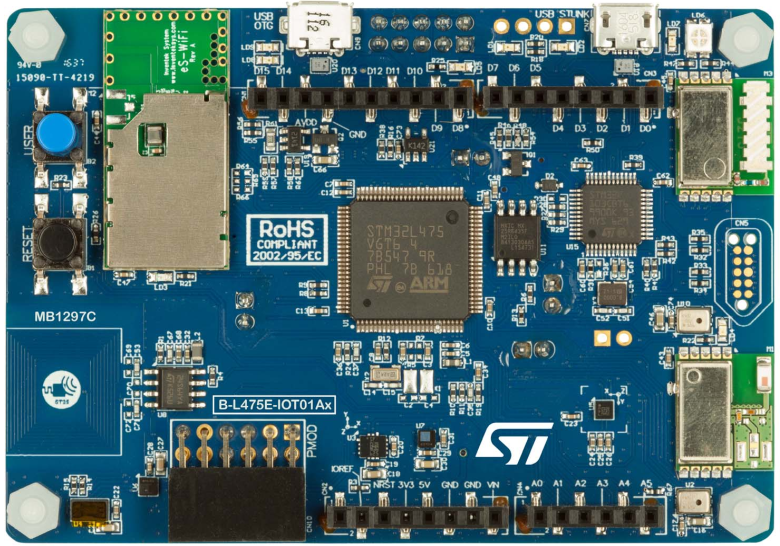
\includegraphics[width=10cm]{source/images/Board}
	\caption{B-L475E-IOT01A Discovery kit \cite{B-L475E-IOT01A}}\label{Node}
\end{figure}


F"ur diese Arbeit werden wir uns auf zwei sensoren beschr"anken. Erstmal den HTS221 Temperatur- und Feuchtigkeitssensor und dann den LSM6DSK 3D Gyroscope und 3D Beschleunigungssesnsor. Diese Daten werden erfasst und drahtlos an dem LoRaWAN-Server "ubertragen. Die folgenden Unterkapitel beschreiben wie diese Sensoren funktionieren und erkl"art wie sie anzusteuern sind, damit die erhaltene Daten n"aherungsweise die Realit"at entsprechen.  

\subsection {HTS221 Temperatursensor}\label{Temp}
In diesem Unterkapitel wird der HTS221 Temperatur- und Feuchtigkeitssensor beschrieben und erkl"art wie die Temeratur und die Feuchtigkeit zu ermitteln sind.

Der HTS221 Sensor misst die relative Feuchtigkeit und die Temperatur und speichert die Daten (16-Bits von Datentyp Integer) als zweierkomplement. Diese Daten k"onnen "uber I2C- oder SPI-Schnittstelle gelesen werden. Die gespeicherte Daten sind Rohdaten, die am Ausgang von dem Analog-Digital-Converter (ADC) verf"ugbar sind (Siehe Abbildung \ref{HT_sensor}). Um die Temperatur in \textdegree{}c und die relative Feuchtigkeit in \% zu bekommen, muss man die Daten aus den Registern konvertieren.

\begin{figure}[h]
	\centering
	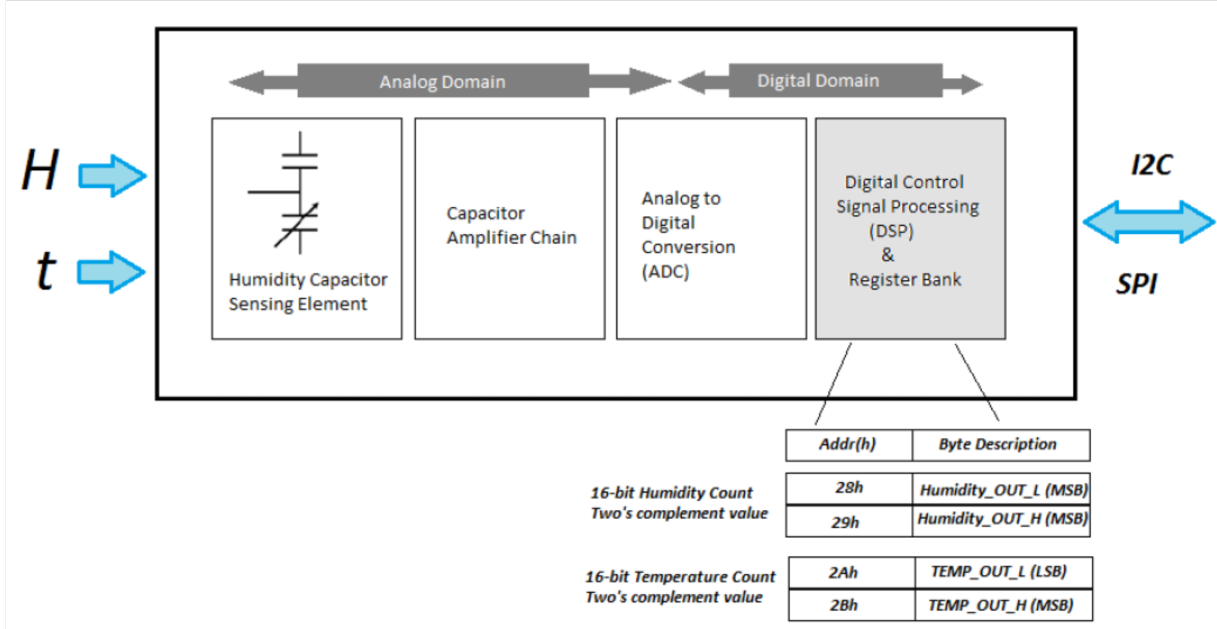
\includegraphics[width=14cm]{source/images/HTS221_sensor}
	\caption{Humidity sensor analog-to-digital flow \cite{HTS221}}\label{HT_sensor}
\end{figure}

\subsubsection{Feuchtigkeit ermitteln}

An dieser Stelle wird erkl"art wie die Feuchtigkeit von dem Sensor ermittet wird. 
Der HTS221 Sensor speichert den Feuchtigkeitswert in Rohz"alungen in zwie 8-Bit-Registern:
\begin{itemize}
	\item H\_OUT\_H (0x29) (H"ochstwertige Bits)
	\item H\_OUT\_L (0x28) (Niedrigswertige Bits)
\end{itemize}
Die zwei Bytes werden verkettet, um ein zweierkomplement dargestelltes 16-Bit Wort zu bilden. Der relative Feuchtigkeitswert muss durch lineare Interpolation
der Register (HUMIDITY\_OUT\_H \& HUMIDITY\_OUT\_L) mit dem Kalibrierregistern berechnet werden.

Der HTS221 Sensor ist bei der Herstellung schon kalibiert und die erforderlichen Koeffizienten sind ADC 16-Bit-Werte, die in den internen register des Sensors zu lesen sind. Eine weitere Kalibrierung durch den Benutzer ist nicht erforderlich.

Die Tabelle \ref{tab:Reg_H} stellt die register dar, in dem die kalibrierwerte gespeichert sind. 

\begin{center}
	\begin{table}[htbp] 
		\centering 
		\Large
	%	\footnote{(u16) 16Bit-Wert ohne Vorzeichen, (s16) 16-Bit-wert mit Vorzeichen}
		\begin{tabular}{l|c|r}
			\textbf{Variable} & 	\textbf{Adresse} & \textbf{Format}\footnotemark\\
			\hline
			H0\_rH\_x2	& 0x30	& u(16) \\
			\hline
			H1\_rH\_x2	& 0x31	& u(16)\\
			\hline
			H0\_TO\_OUT\_H & 0x36	& s(16)\\
			\hline
			H0\_TO\_OUT\_L 	& 0x37  & s(16)\\
			\hline
			H1\_TO\_OUT\_H	& 0x3A	& s(16)\\
			\hline
			H1\_TO\_OUT\_L 	& 0x3B  & s(16)\
		\end{tabular} 
		\caption{Kalibrierregister fur relative Feuchtigkeit} 
		\label{tab:Reg_H} 
		 
	\end{table}
\end{center}
\footnotetext{(u16) 16Bit-Wert ohne Vorzeichen, (s16) 16-Bit-wert mit Vorzeichen}

Nun wissen wir welche Registerzu lesen sind, damit die relative Feuchtigkeit mit Hilfe der Interpolation berechnet wird. Die folgenden Schritten mussen vor der Berechnung durchgef"uhrt werden:

\begin{itemize}
	\item Werte von H0\_rH\_x2 und H1\_rH\_x2 aus Registern 0x30 und 0x31 lesen 
	\item H0\_rH\_x2 und H1\_rH\_x2 durch zwei teilen
	\item Werte von H0\_TO\_OUT aus Registern 0x36 und 0x37 lesen 
	\item Werte von H1\_TO\_OUT aus Registern 0x3A und 0x3B lesen
	\item Rohdate von H\_T\_OUT aus Registern 0x28 und 0x29 lesen
\end{itemize}

Nach dem diese Register gelesen wurden, kann nun die Berechnung der relative Feuchtigkeit erfolgen. 

\begin{figure}[h]
	\centering
	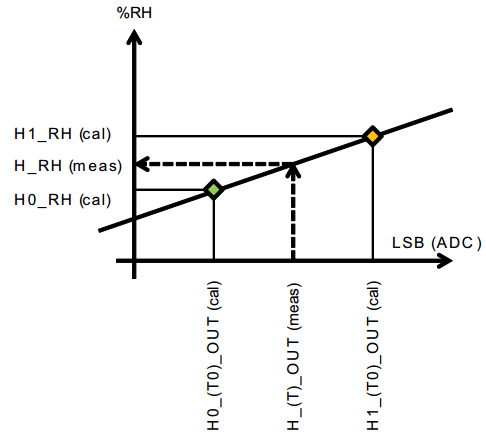
\includegraphics[width=10cm]{source/images/rH}
	\caption{Linear interpolation to convert LSB to rH \% \cite{HTS221}}\label{graph:rH}
\end{figure}

Aus Abbildung \ref{graph:rH} bekommt man mit Interpolation die folgende Formel:

\[
RH\% = \frac{((H1\_rH - H0\_rH) . (H\_T\_OUT - H0\_T0\_OUT))}{(H1\_T0\_OUT - H1\_T0\_OUT) } + H0\_rH 
\]

Da die kalibrierwerten bei der Herstellung des Bausteins schon festgesetzt sind, soll man die Kalibrierregister bei der Programmierung nur ein mal auslesen, dies ersparrt den Rechenaufwand des Mikrocontrollers. 

\subsubsection{Temperatur ermitteln}
Der HTS221 Sensor speichert die Temperaturwerten in Rohz"alungen in zwie 8-Bit-Registern:

\begin{itemize}
	\item T\_OUT\_H (0x2A) (H"ochstwertige Bits)
	\item T\_OUT\_L (0x2B) (Niedrigswertige Bits)
\end{itemize}



\subsection{LSM6DSL 3D Gyroscope und 3D Beschleunigungssensor}\label{Acc/Gy}


\section{LoRa Node: i-nucleo-lrwan1}\label{LoRa Modul}
\subsection{LoRaWAN Protokol}\label{LoRaWAN_P}
\subsection{AT Commandos}\label{AT}


\chapter{Gateway und LoRaWAN server}\label{G_S}

\section{Gateway}\label{Gateway}
\section{Server}\label{server}
